\section{Description des états}

Un état du jeu est formé par un ensemble d’éléments fixes sur le terrain et un ensemble
d’éléments mobiles ainsi que l'état du joueur. 


\begin{itemize}
\item Nom,
\item Position
\end{itemize}

\subsection{États éléments fixes}

La map est formé par une grille d’éléments nommé « Map ». La taille de cette grille est
fixée. Les éléments fixes sur cette grille sont :\\

\begin{itemize}
\item L'élément "StellarSystem". Les systèmes stellaires sont des éléments
fixes que le joueur pourra coloniser. Ils sont composés de 1 à 4 planètes, il existe 3 types de planètes :\\

\begin{itemize}
\item les planètes "Neutral" qui ont une répartition des ressources équilibré
\item les planètes "Hot" qui favorisent la ressource de production
\item les planètes "Cold" qui favorisent la ressource de science
\end{itemize}\\

De plus lorsqu'un joueur possède une système stellaire, il a la possibilité de construire des bâtiments qui seront liés au système. Ces derniers produiront une quantité différente des 4 ressources\\





\item L'élément "StellarWay". Ce sont des routes de l'espace qui relient deux systèmes stellaires entre eux. Sa longueur influera sur le temps qu'un vaisseau mettra à la parcourir entièrement.
\end{itemize}

\subsection{États éléments mobiles}

Les seuls éléments mobiles du jeu sont les vaisseaux.

L'élément mobile "Ship" est dirigé par le "Player", il est construit ou acheter dans les stystèmes stellaires. Chaque « Ship » possède des statistiques propres à sa classe. On lui associe ainsi des points de vie “heath”, des dégats d'attaque “attack-point”, une défense “defense-point” et des points de déplacement. Chaque vaisseaux possède aussi un avantage parmis ses quatres:\\

\begin{itemize}
\item Dégât augmenté contre les vaisseaux,
\item Dégât augmenté contre les bâtiments,
\item Vitesse de déplacement augmenté,
\item Possibilité de coloniser.
\end{itemize}
Les vaisseaux possèdent un niveau qui augmente leurs statistiques, ses niveaux sont gagnés lors de victoires contre un vaisseau ennemie. 

\subsection{État du joueur}

Le joueur possède un ensemble d'élément fixe, les systèmes stellaires, et mobile, les vaisseaux, ainsi que des ressource qu'il gagne à chaque tours de jeu.

\section{Conception logiciel}

L'architecture du diagramme de classe est fondée sur le Polymorphisme par sous-typage dont la classe “Objet” est la classe mère.
Toute la hiérarchie des classes filles “Objet” permettent de représenter les différentes
catégories et types d’élément.
\begin{figure}[!h]
\centering
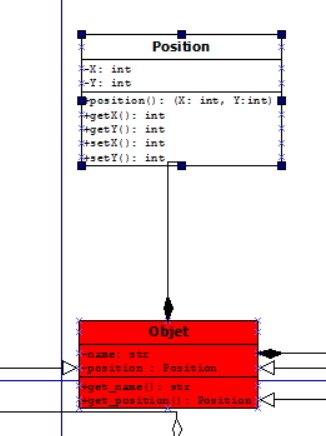
\includegraphics[width=0.5\textwidth]{pics/classe_objet.PNG}
\caption[Bloc "Objet"]{\label{figure_simple}Bloc "Objet"}
\end{figure}

On peut distinguer les classes filles qui héritent directement de la classe “Objet” :

\begin{itemize}
    \item La classe "Ship" est la classe qui contient toutes les informations des vaisseaux. Chaque vaisseau est associé des statistiques.  On associe
également par relation de composition une struture “ShipStats” décrivant
le type de vaisseau, ainsi qu’une énumération “Ship-TypeID” exposant sa
classe de vaisseau.
\begin{figure}[!h]
\centering
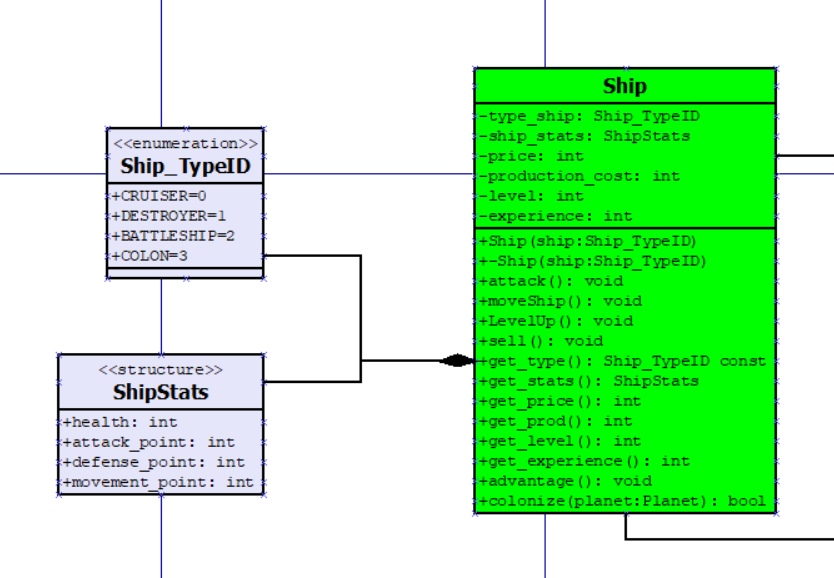
\includegraphics[width=0.8\textwidth]{pics/classe_vaisseau.PNG}
\caption[Bloc "Ship"]{\label{figure_simple}Bloc "Ship"}
\end{figure}

\item La classe "StellarSytem" est la classe qui contient toutes les informations sur les systèmes stellaires. \\

\begin{figure}[!h]
\centering
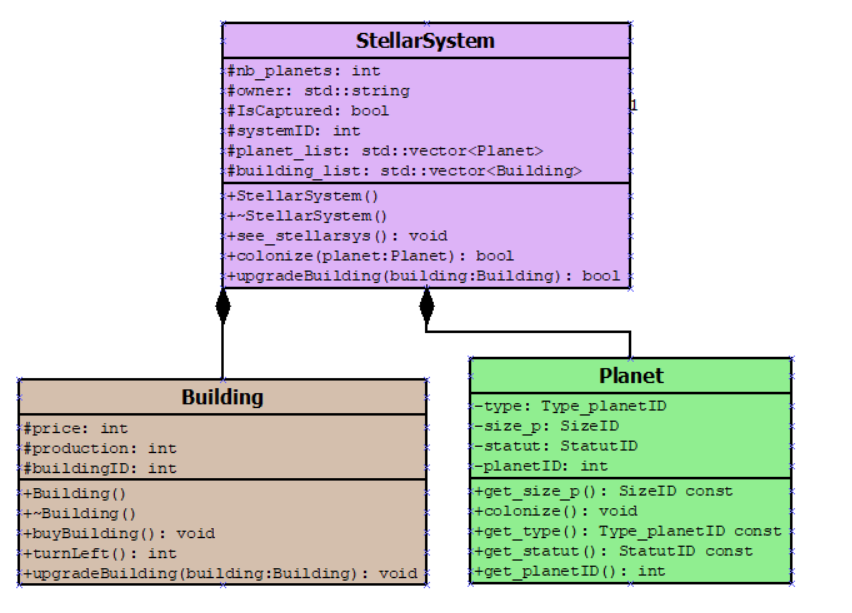
\includegraphics[width=0.6\textwidth]{pics/classe_system.PNG}
\caption[Bloc "StellarSytem"]{\label{figure_simple}Bloc "StellarSytem"}
\end{figure}

Elle associé à deux sous classes "Building" et "Planet"\\

\begin{figure}[!h]
\centering
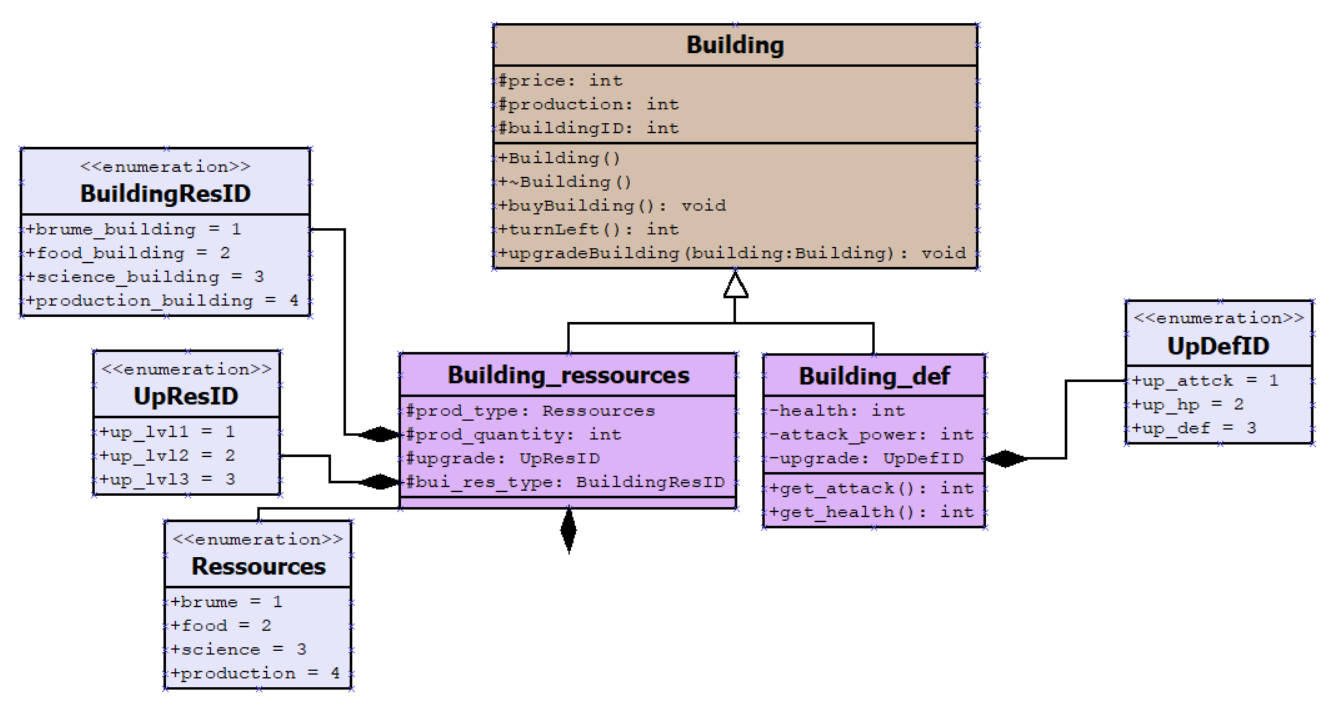
\includegraphics[width=0.6\textwidth]{pics/classe_batiment.PNG}
\caption[Bloc "Building"]{\label{figure_simple}Bloc "Building"}
\end{figure}

\begin{figure}[!h]
\centering
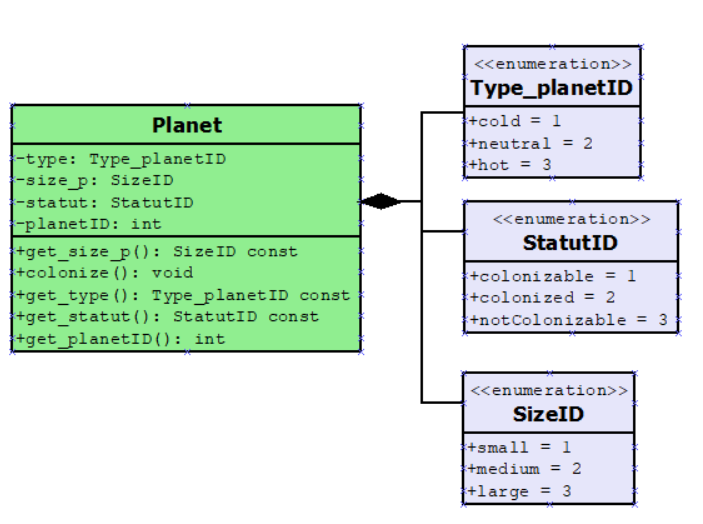
\includegraphics[width=0.6\textwidth]{pics/classe_planet.PNG}
\caption[Bloc "Planet"]{\label{figure_simple}Bloc "Planet"}
\end{figure}

\item la classe "Map" établit aussi une relation d'héritage

\begin{figure}[!h]
\centering
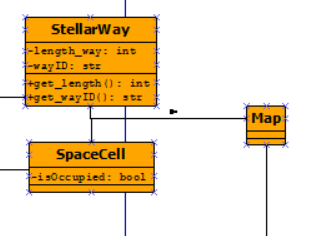
\includegraphics[width=0.6\textwidth]{pics/classe_map.PNG}
\caption[Bloc "Map"]{\label{figure_simple}Bloc "Map"}
\end{figure}
\end{itemize}

la classe " Player" est la classe qui va centraliser l'ensemble des informations concernant le joueur. Le joueur se voit associé des vaisseaux, des systèmes stellaires, des batiments,.. Il possède aussi diffèrent type de ressources, " Ressource", qu'il produit à chaque tours et un arbre de technologie,  "TechnologyTree" où il pourra faire des recherches pour améliorer ses vaisseaux ou bâtiments. 

\begin{figure}[!h]
\centering
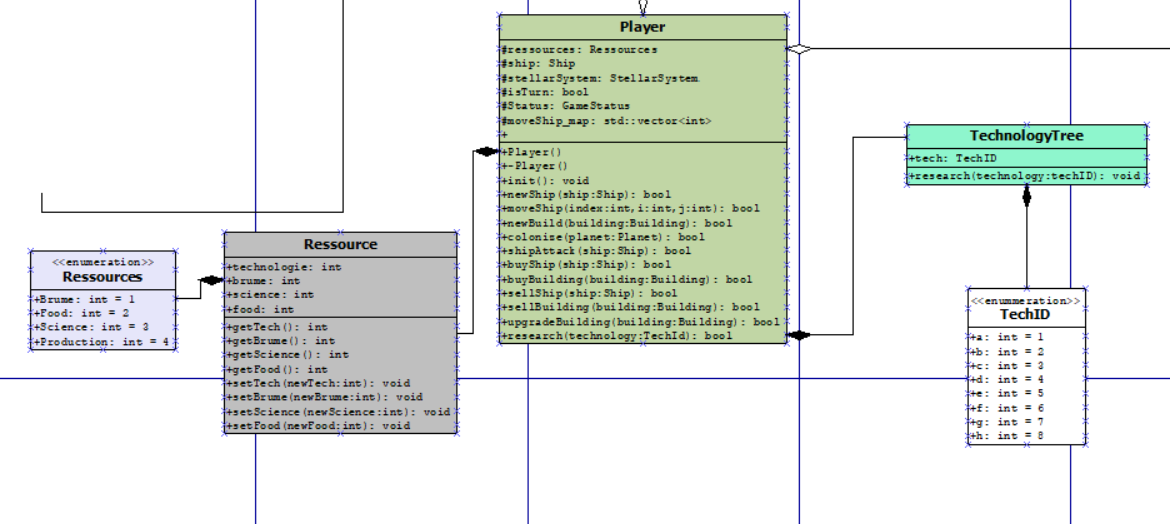
\includegraphics[width=0.8\textwidth]{pics/classe_player.PNG}
\caption[Bloc "Player"]{\label{figure_simple}Bloc "Player"}
\end{figure}

Finalement nous avons la classe "State" qui contient la classe "Player" et "Map".


\begin{figure}[!h]
\centering
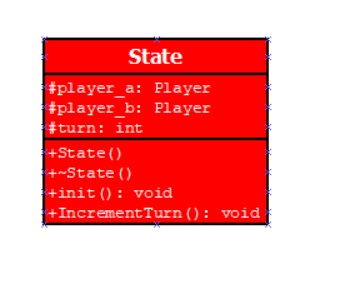
\includegraphics[width=0.3\textwidth]{pics/classe_state.PNG}
\caption[Bloc "State"]{\label{figure_simple}Bloc "State"}
\end{figure}

\begin{figure}[!h]
\centering
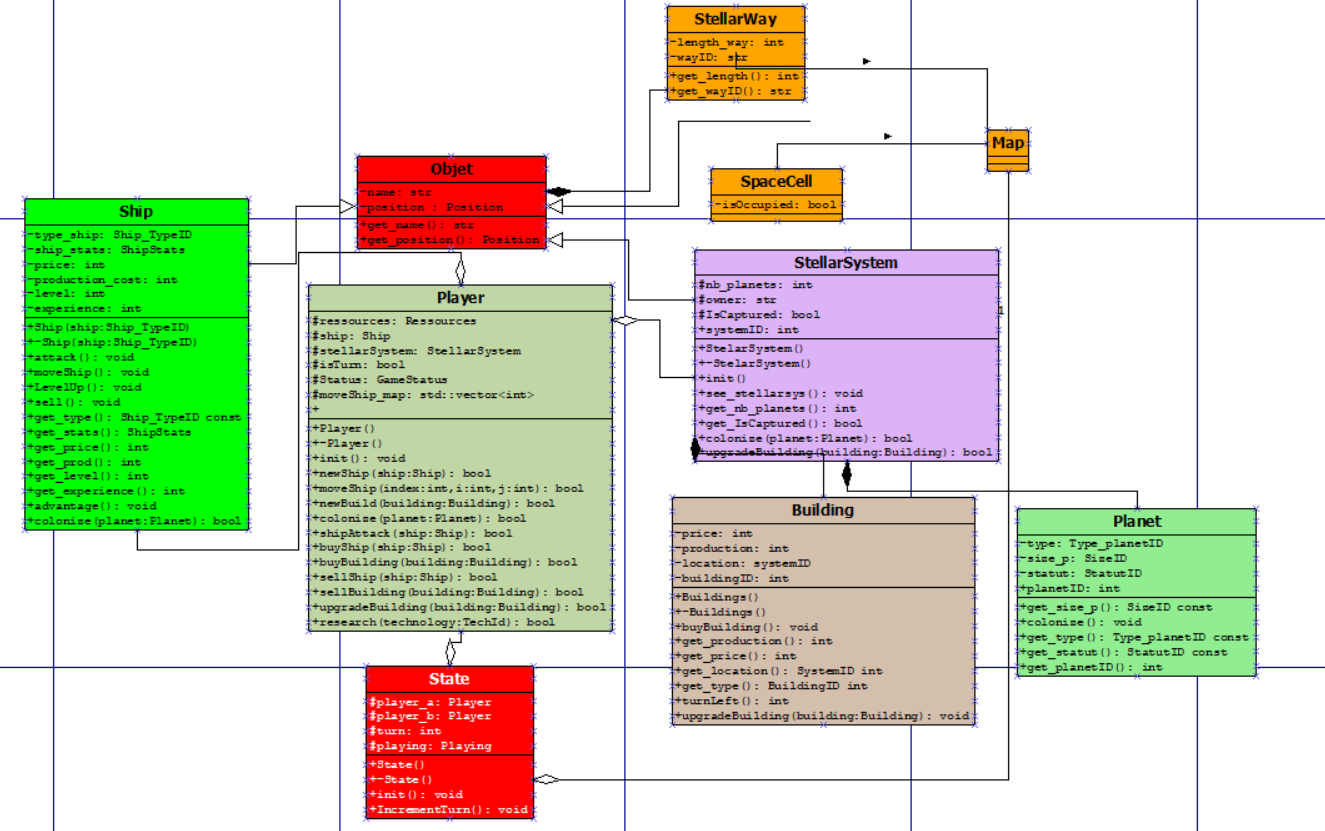
\includegraphics[width=1\textwidth]{pics/ensemble_classe.PNG}
\caption[State diagram]{\label{figure_simple}State diagram}
\end{figure}